\documentclass[usenatbib,fleqn]{mnras}

\pdfoutput=1

\usepackage{amsmath}
\usepackage{amssymb}
\usepackage{blindtext}
\usepackage{bm}
\usepackage{color}
\usepackage{graphicx}
\usepackage{hyperref}
\usepackage[all]{hypcap}
% \usepackage{lineno}
\usepackage{longtable}
\usepackage{multicol}
\usepackage{multirow}
\usepackage{natbib}
% \usepackage{flushend}
\usepackage{txfonts}
\usepackage{wasysym}
\usepackage[capitalize,nameinlink]{cleveref}

% cleveref tweak to remove parentheses from equations
\creflabelformat{equation}{#2#1#3}
\crefrangelabelformat{equation}{#3#1#4 to #5#2#6}

% For links of references
\hypersetup{colorlinks,
  linkcolor=red,
  filecolor=red,
  urlcolor=magenta,
  citecolor=blue}

\usepackage{array}
\newcolumntype{L}[1]{>{\raggedright\let\newline\\\arraybackslash\hspace{0pt}}m{#1}}
\newcolumntype{C}[1]{>{\centering\let\newline\\\arraybackslash\hspace{0pt}}m{#1}}
\newcolumntype{R}[1]{>{\raggedleft\let\newline\\\arraybackslash\hspace{0pt}}m{#1}}

\newcommand{\comment}[1]{\textbf{\color{magenta} #1}}

\newcommand{\eagle}{EAGLE}
\newcommand{\hbt}{\textsc{hbt+}}

\newcommand{\msub}{m_\mathrm{sub}}
\newcommand{\Mhost}{M_\mathrm{host}}
\newcommand{\mstar}{m_\star}
\newcommand{\Msun}{\mathrm{M}_\odot}
\newcommand{\Mtotal}{M_\mathrm{total}}
\newcommand{\mtwo}{M_\mathrm{200m}}
\newcommand{\mtwoc}{M_\mathrm{200c}}
\newcommand{\hMsun}{h^{-1}\,\Msun}
\newcommand{\hMpc}{h^{-1}\,\mathrm{Mpc}}
\newcommand{\subfind}{\textsc{subfind}}
\newcommand{\tcent}{t_\mathrm{cent}}
\newcommand{\tinfall}{t_\mathrm{infall}}
\newcommand{\zcent}{z_\mathrm{cent}}
\newcommand{\zinfall}{z_\mathrm{infall}}


\title[Mass content of \eagle\ cluster galaxies]{The history and mass content of cluster galaxies in the \eagle\ simulation}

\author[C.\ Sif\'on et al.]{Crist\'obal Sif\'on$^1$, ...
\\
$^1$Instituto de F\'isica, Pontificia Universidad Cat\'olica de Valpara\'iso, Casilla 4059, Valpara\'iso, Chile
}

% These dates will be filled out by the publisher
% \date{Accepted XXX. Received YYY; in original form ZZZ}

% Enter the current year, for the copyright statements etc.
\pubyear{2019}

\begin{document}
\label{firstpage}
\pagerange{\pageref{firstpage}--\pageref{lastpage}}

% \linenumbers

\maketitle

\begin{abstract}
%  We use the upgraded Hierarchical Bound Tree (HBT+) subhalo catalogue from the \eagle\ cosmological hydrodynamical simulation to explore the effects of  of galaxies into massive ($M_{200m}>10^{13}\,\Msun$) galaxy groups and clusters.
We explore the mass content of cluster galaxies in the \eagle\ cosmological hydrodynamical simulation. 
  
  We explore changes in satellite stellar mass/halo mass as a function of (the observationally accessible) distance from host/nearest cluster, as well as the more physical change as a function of time for the same satellites.
  
  We identify the progenitors of $z=0$ satellites as \textbf{some population of centrals at some earlier time}, and find \textbf{the following problems arise when interpreting differences between present-day satellites with present-day centrals}

\end{abstract}



\section{Wish/thought list}


\comment{are all quantities in the HBT catalogs in units of $h$, or is the value of $h$ already included?}
\\

(Given in the order they came to my head)

\begin{enumerate}
  \item Explore what difference does it make where did the satellite come from, by binning as a function of cluster-centric distance but also, for galaxies not part of the cluster, by host mass (probably do not need groups less massive than $10^{12}\,h^{-1}\,\Msun$, as that's already the mass of the Milky Way). Another way is, for galaxies not part of a massive cluster, to see how far they are to a massive cluster and what is their host mass. For a given distance to a massive cluster, does the mass relation change with host mass? We may need to control by distance from host center as well, and then it may become too noisy...
  \item try to find a good definition for subhalo size using the density profiles. Perhaps differences between our measurements and \eagle\ are caused by a model error?
  \item Plot stellar-to-total mass \emph{ratios} as a function of cluster-centric distance.
  \item When plotting ``distance to nearest cluster'' as opposed to distance to \emph{host} cluster, should 
  \item Use some definition of ``phase-space distance'', similar to the bins in Fig 1 of Muzzin+14.
\end{enumerate}

\subsection{Literature notes}

\begin{enumerate}
  \item \citet{rhee17}: weak preprocessing in general ($<30\%$ mass loss prior to entering cluster). Mass lost up to 1st pericenter $\sim$20-30\%, constant with time (Fig 4)
\end{enumerate}

\subsection{New thoughts emerging from my \hbt\ exploration:}
\begin{enumerate}
  \item To see what produces changes (especially fluctuations) in mass, should look at the location of the (sub)halo and its neighbors. It's probably that their spiraling into each other or so.
\end{enumerate}



\section{Introduction}

Over time, galaxies evolve and co-evolve as they are pulled together by gravity and form larger gravitationally-bound systems such as groups and clusters of galaxies, and eventually merge into larger galaxies. This hierarchical formation scenario is widely supported by simulations of structure formation \citep[e.g.,][]{?} and observations \citep[e.g.,][]{?}. Galaxies, in turn, reside in dark matter subhaloes, which interact gravitationally to form ever larger subhaloes and haloes (where subhaloess

In this paper, we study the demographics and evolution of satellite galaxies and their host haloes in detail, paying particular attention to the transfer of mass from galaxies to their host groups and clusters, 

In this paper we refer generically to ``galaxy groups'' as all galaxy associations more massive than $\mtwo=10^{11}\,\Msun$, and to ``clusters'' as the subset of those groups which have $\mtwo>10^{13}\,\Msun$. (This is a more relaxed definition of ``cluster'' than usual.) Throughout, we refer to masses $M_{\Delta m}$ ($M_{\Delta c}$) as the mass containing $\Delta$ times the mean (critical) density of the Universe at the group redshift. Where appropriate, we adopt the cosmology used in the \eagle\ simulations,  with \textbf{parameters...}
%
Throughout, we use $\log$ to refer to base 10-logarithm.


\section{Simulation}

We use the Evolution and Assembly of Galaxies and their Environment (\eagle) simulations \citep{schaye15,crain15}. \eagle\ is a suite of cosmological hydrodynamical simulations with varying box sizes, resolutions, and baryonic feedback prescriptions. The simulation we use here is labelled \texttt{RefL0100N1504} and has a box size of $(100\,\hMpc)^3$, with N particles and mass resolutions of X,Y,Z for dark matter, gas and stars, respectively. Our study is based on the upgraded Hierarchical Bound Tree \citep[\hbt,][]{han18} post-processing of \eagle, in which subhaloes are found ... . 

\comment{Here, we consider all subhaloes with masses $\msub\geq XXX \Msun$ residing in haloes with masses $\Mhost\geq10^{11}\Msun$.}

\begin{figure}
  \centerline{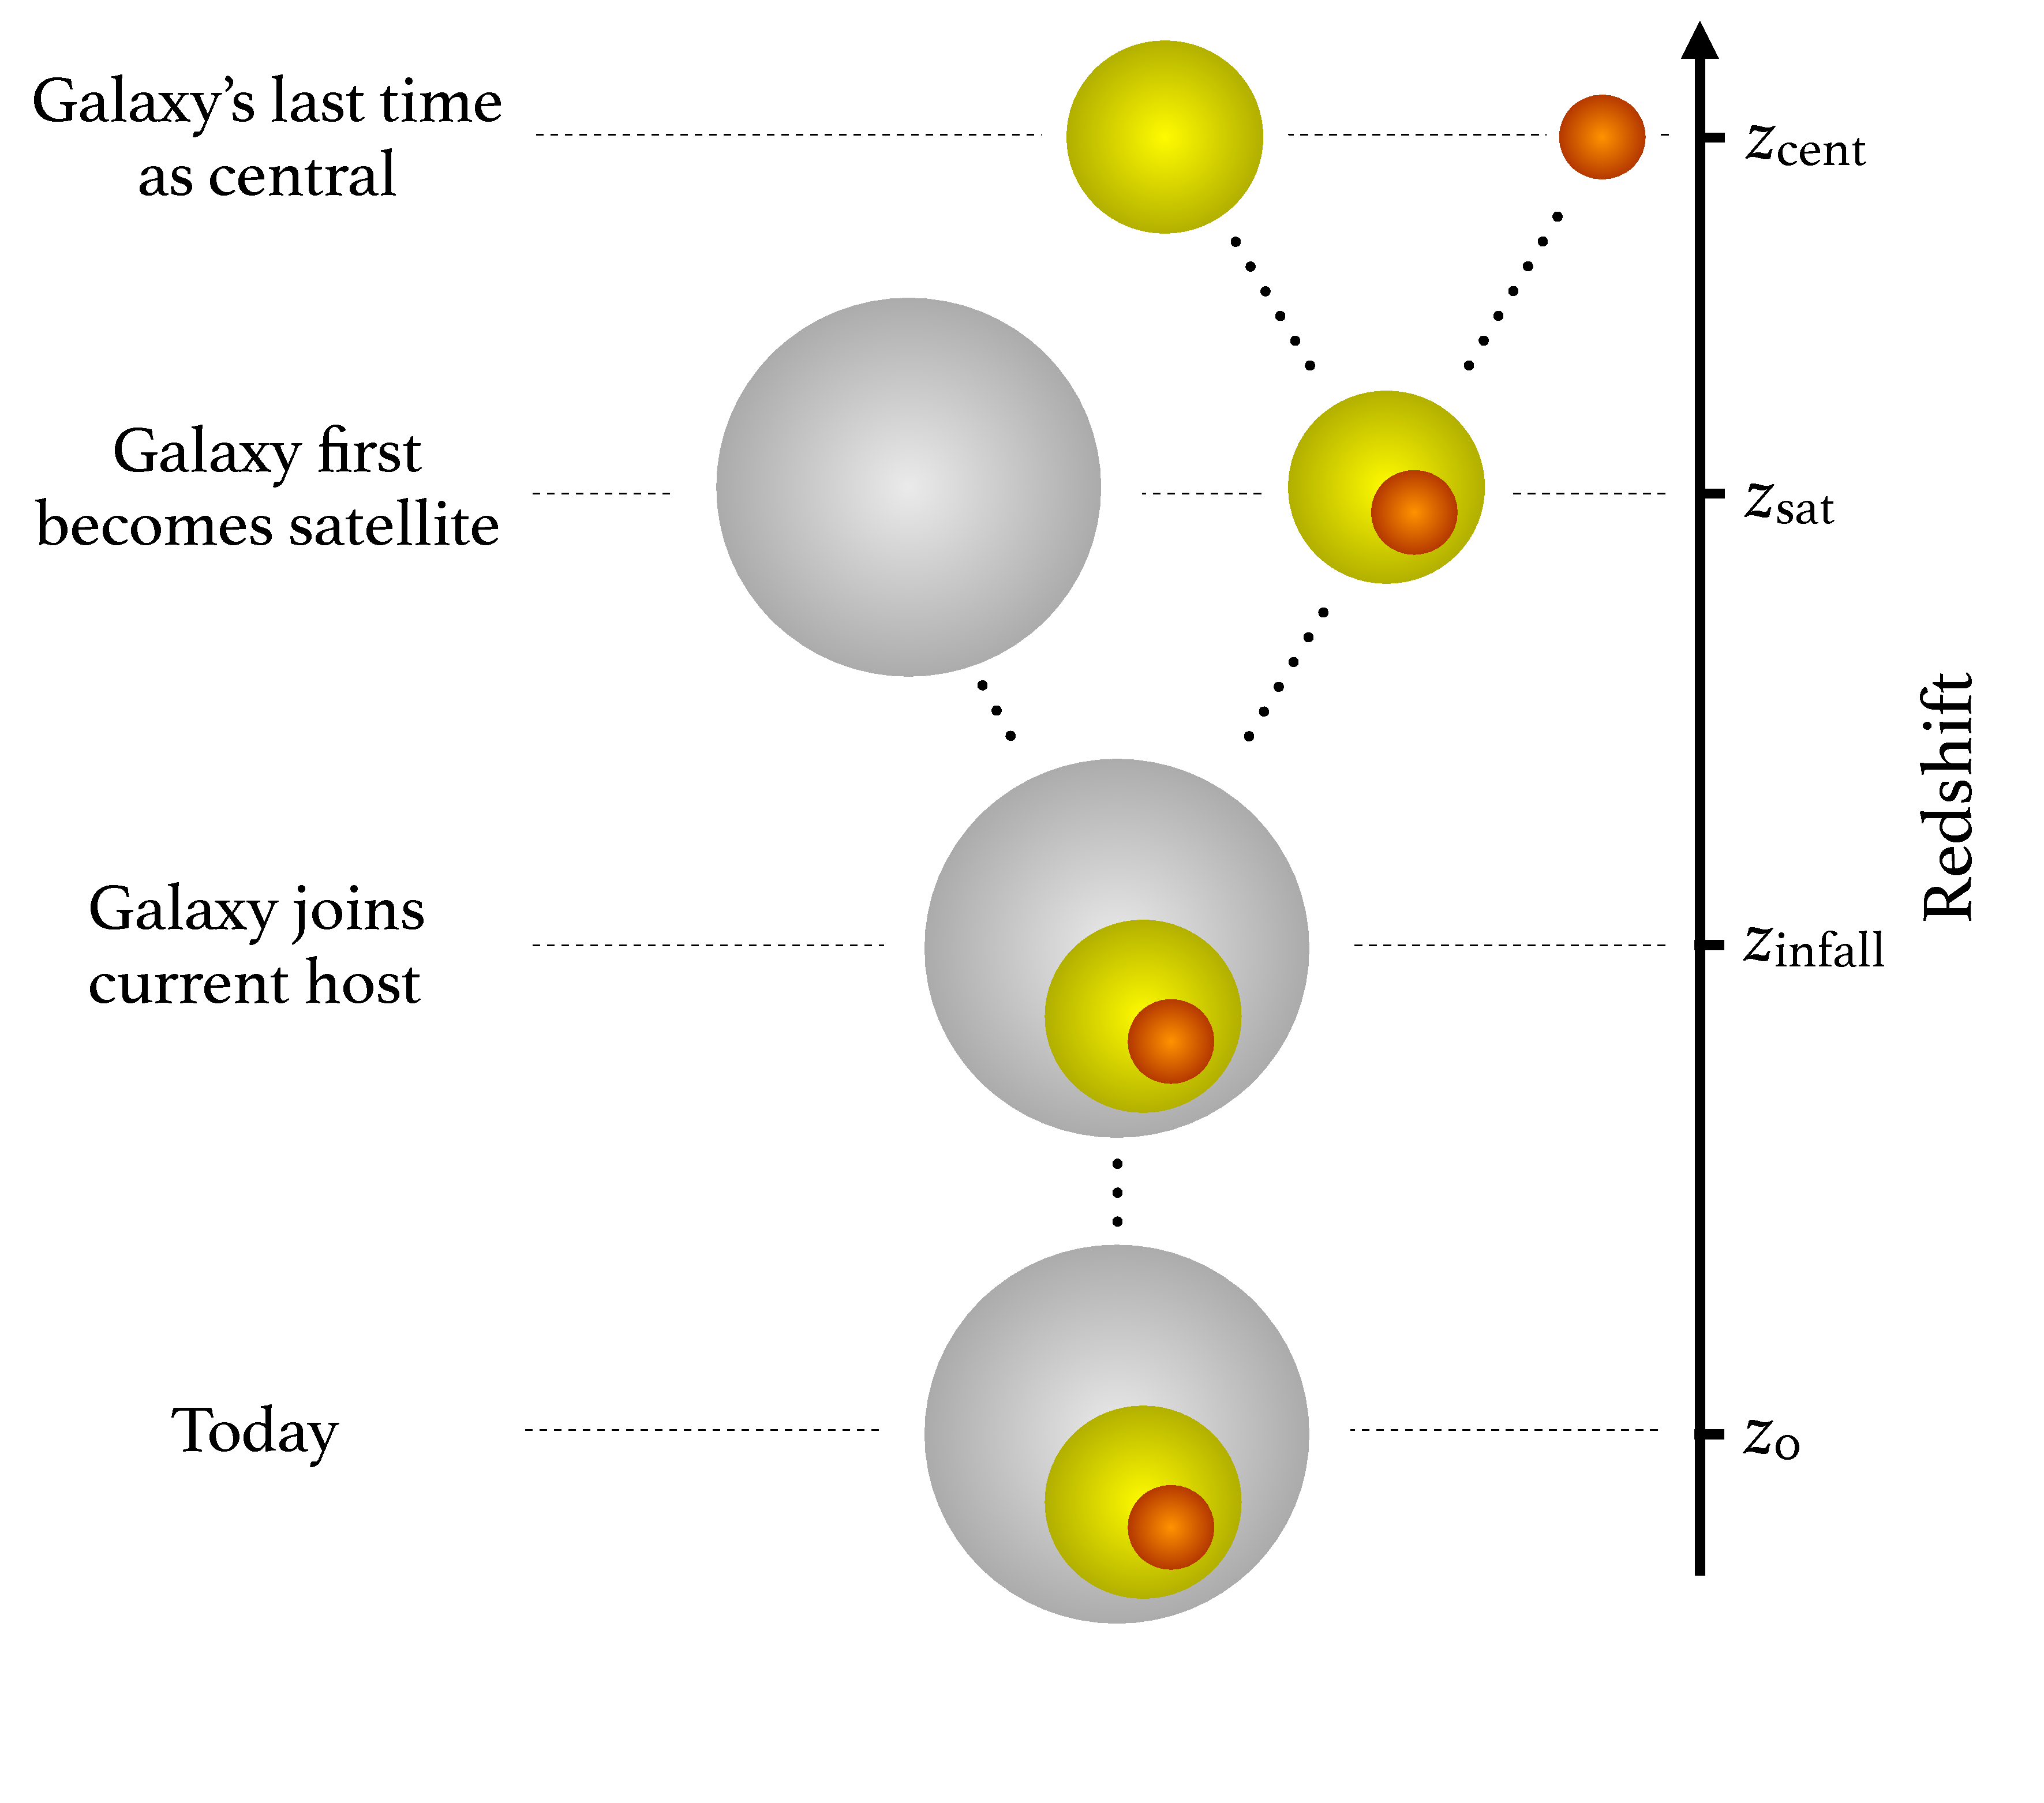
\includegraphics[width=\linewidth]{history_chart.pdf}}
  \caption{Schematic figure showing the relevant times we consider in this work. The brown circle represents a galaxy of interest, 
which is a satellite at redshift $z_0$, part of a host group shown in grey. We identify the last redshift (earliest time) at which the brown
satellite was hosted by the grey host as $\zinfall$. The last time at which the brown satellite was a central galaxy is labelled
$\zcent$. When the brown satellite fell into the grey host (identified at present with \texttt{GroupID}), it may in fact have
already been part of another group, shown in green. If this is the case, then $\zcent \neq \zinfall$. We identify $t_\mathrm{cent}$ and $t_\mathrm{sat}$ separately because a small fraction of subhaloes are labelled as satellites and later re-labelled as centrals, in which case $t_\mathrm{cent} > t_\mathrm{sat}$.}
  \label{fig:chart}
\end{figure}


\subsection{Mass definitions}

Throughout this work we speak of `subhaloes' as all dark matter haloes that inhabit a larger halo, including central subhaloes; and of `galaxies' as the subset of subhaloes which contain at least one star particle. Total masses of both subhaloes and galaxies are  defined as the total mass of all bound particles (i.e., the sum of all dark matter, gas, star, and black hole particles, defined in \hbt\ as \texttt{Mbound}), and stellar masses are similarly defined as the total mass in all bound star particles according to \hbt. Central and satellite subhaloes are hosted within a `host halo', whose total mass is defined as an overdensity mass $M_\Delta$, where in this work $\Delta=\{200,500\}$, and the overdensity is with respect to either the mean density (denoted, e.g., $\mtwo$) or the critical density (e.g., $\mtwoc$), both defined at the corresponding redshift.

We compare the different mass definitions, and show the relative contribution of each to their host halo, in \Cref{f:massdef}.  ...

We show the mass functions for subhaloes and galaxies in \Cref{f:massfunction}.

\begin{itemize}
  \item plot mass functions for different host mass definitions (Mbound, M200Mean, etc) and for subhaloes
  \item show plots comparing those masses directly
\end{itemize}

\begin{figure}
  \centerline{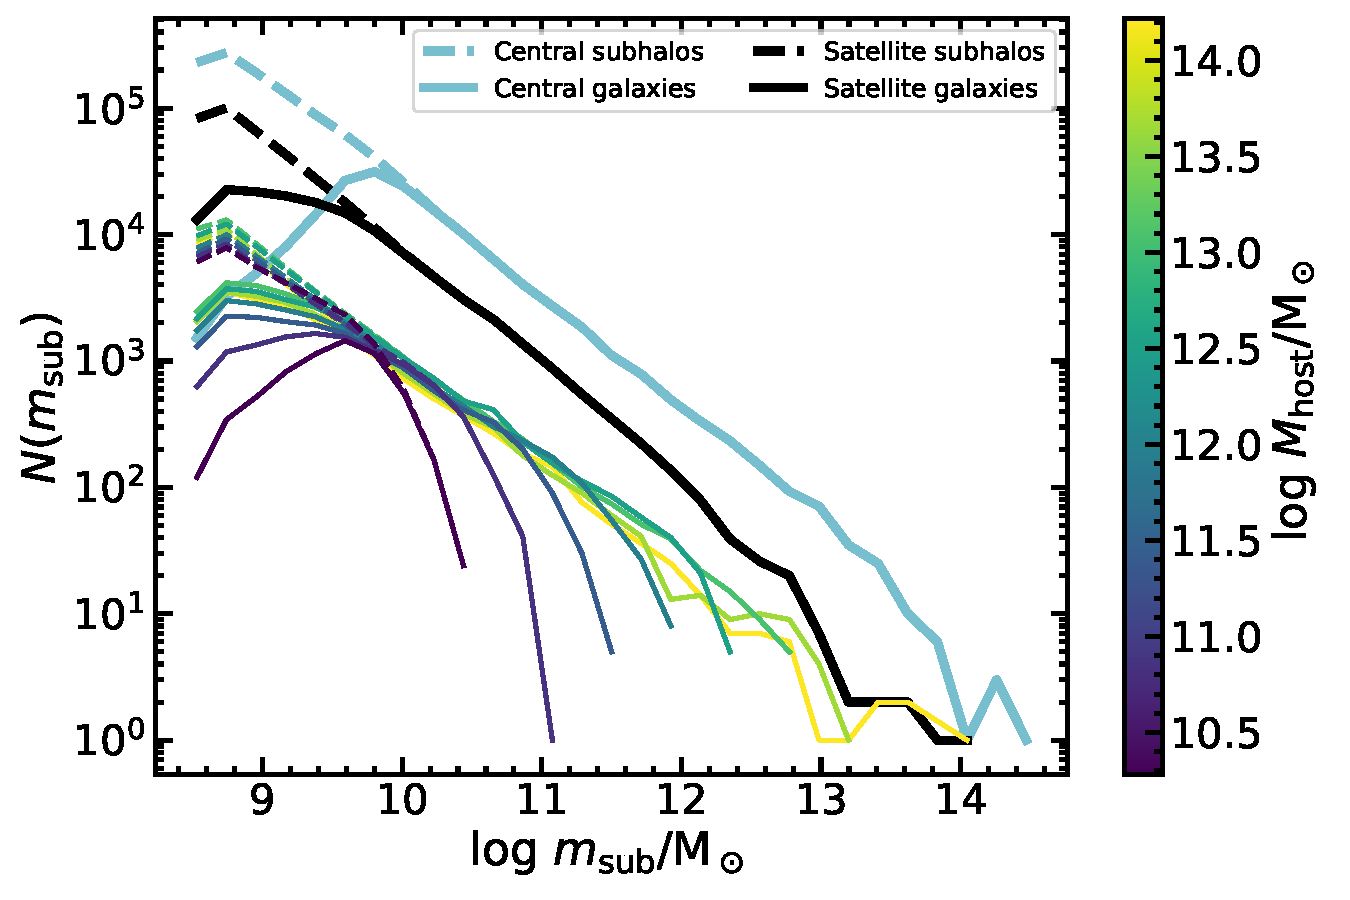
\includegraphics[width=\linewidth]{nmsub.pdf}}
  \caption{Total mass function of central (cyan) and satellite (black) subhaloes (dashed) and galaxies (solid). The thinner, colored lines show the satellite subhalo mass function split into different host halo masses. The rapid drop in each colored curve happens as subhalo masses approach their host halo mass, as the latter is always larger. \comment{Our analysis throughout refers to subhaloes with $\log\msub\geq10.0$, identified by the vertical dotted line.} Here, $\Mhost=\mtwo$.}
  \label{f:massfunction}
\end{figure}


%\begin{figure}
%  \centerline{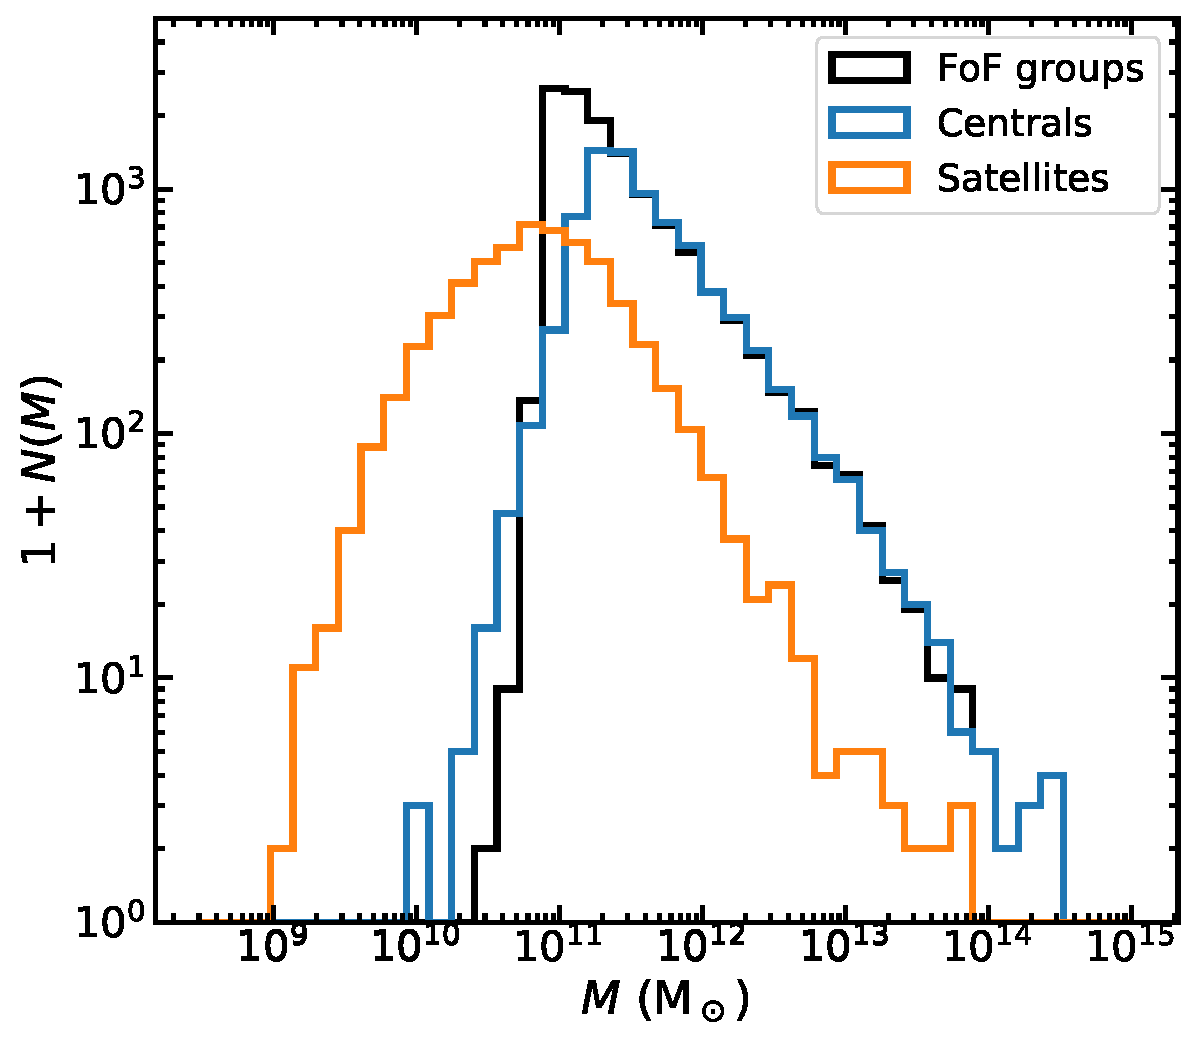
\includegraphics[width=\linewidth]{massfunction.pdf}}
%\caption{Mass function of galaxy groups with $M_{200m}>10^{11}\,\hMsun$ and central and satellite galaxies in the \eagle\ RefL0100N1504 simulation.}
%\label{f:massfunction}
%\end{figure}



%\begin{figure}
%  \centerline{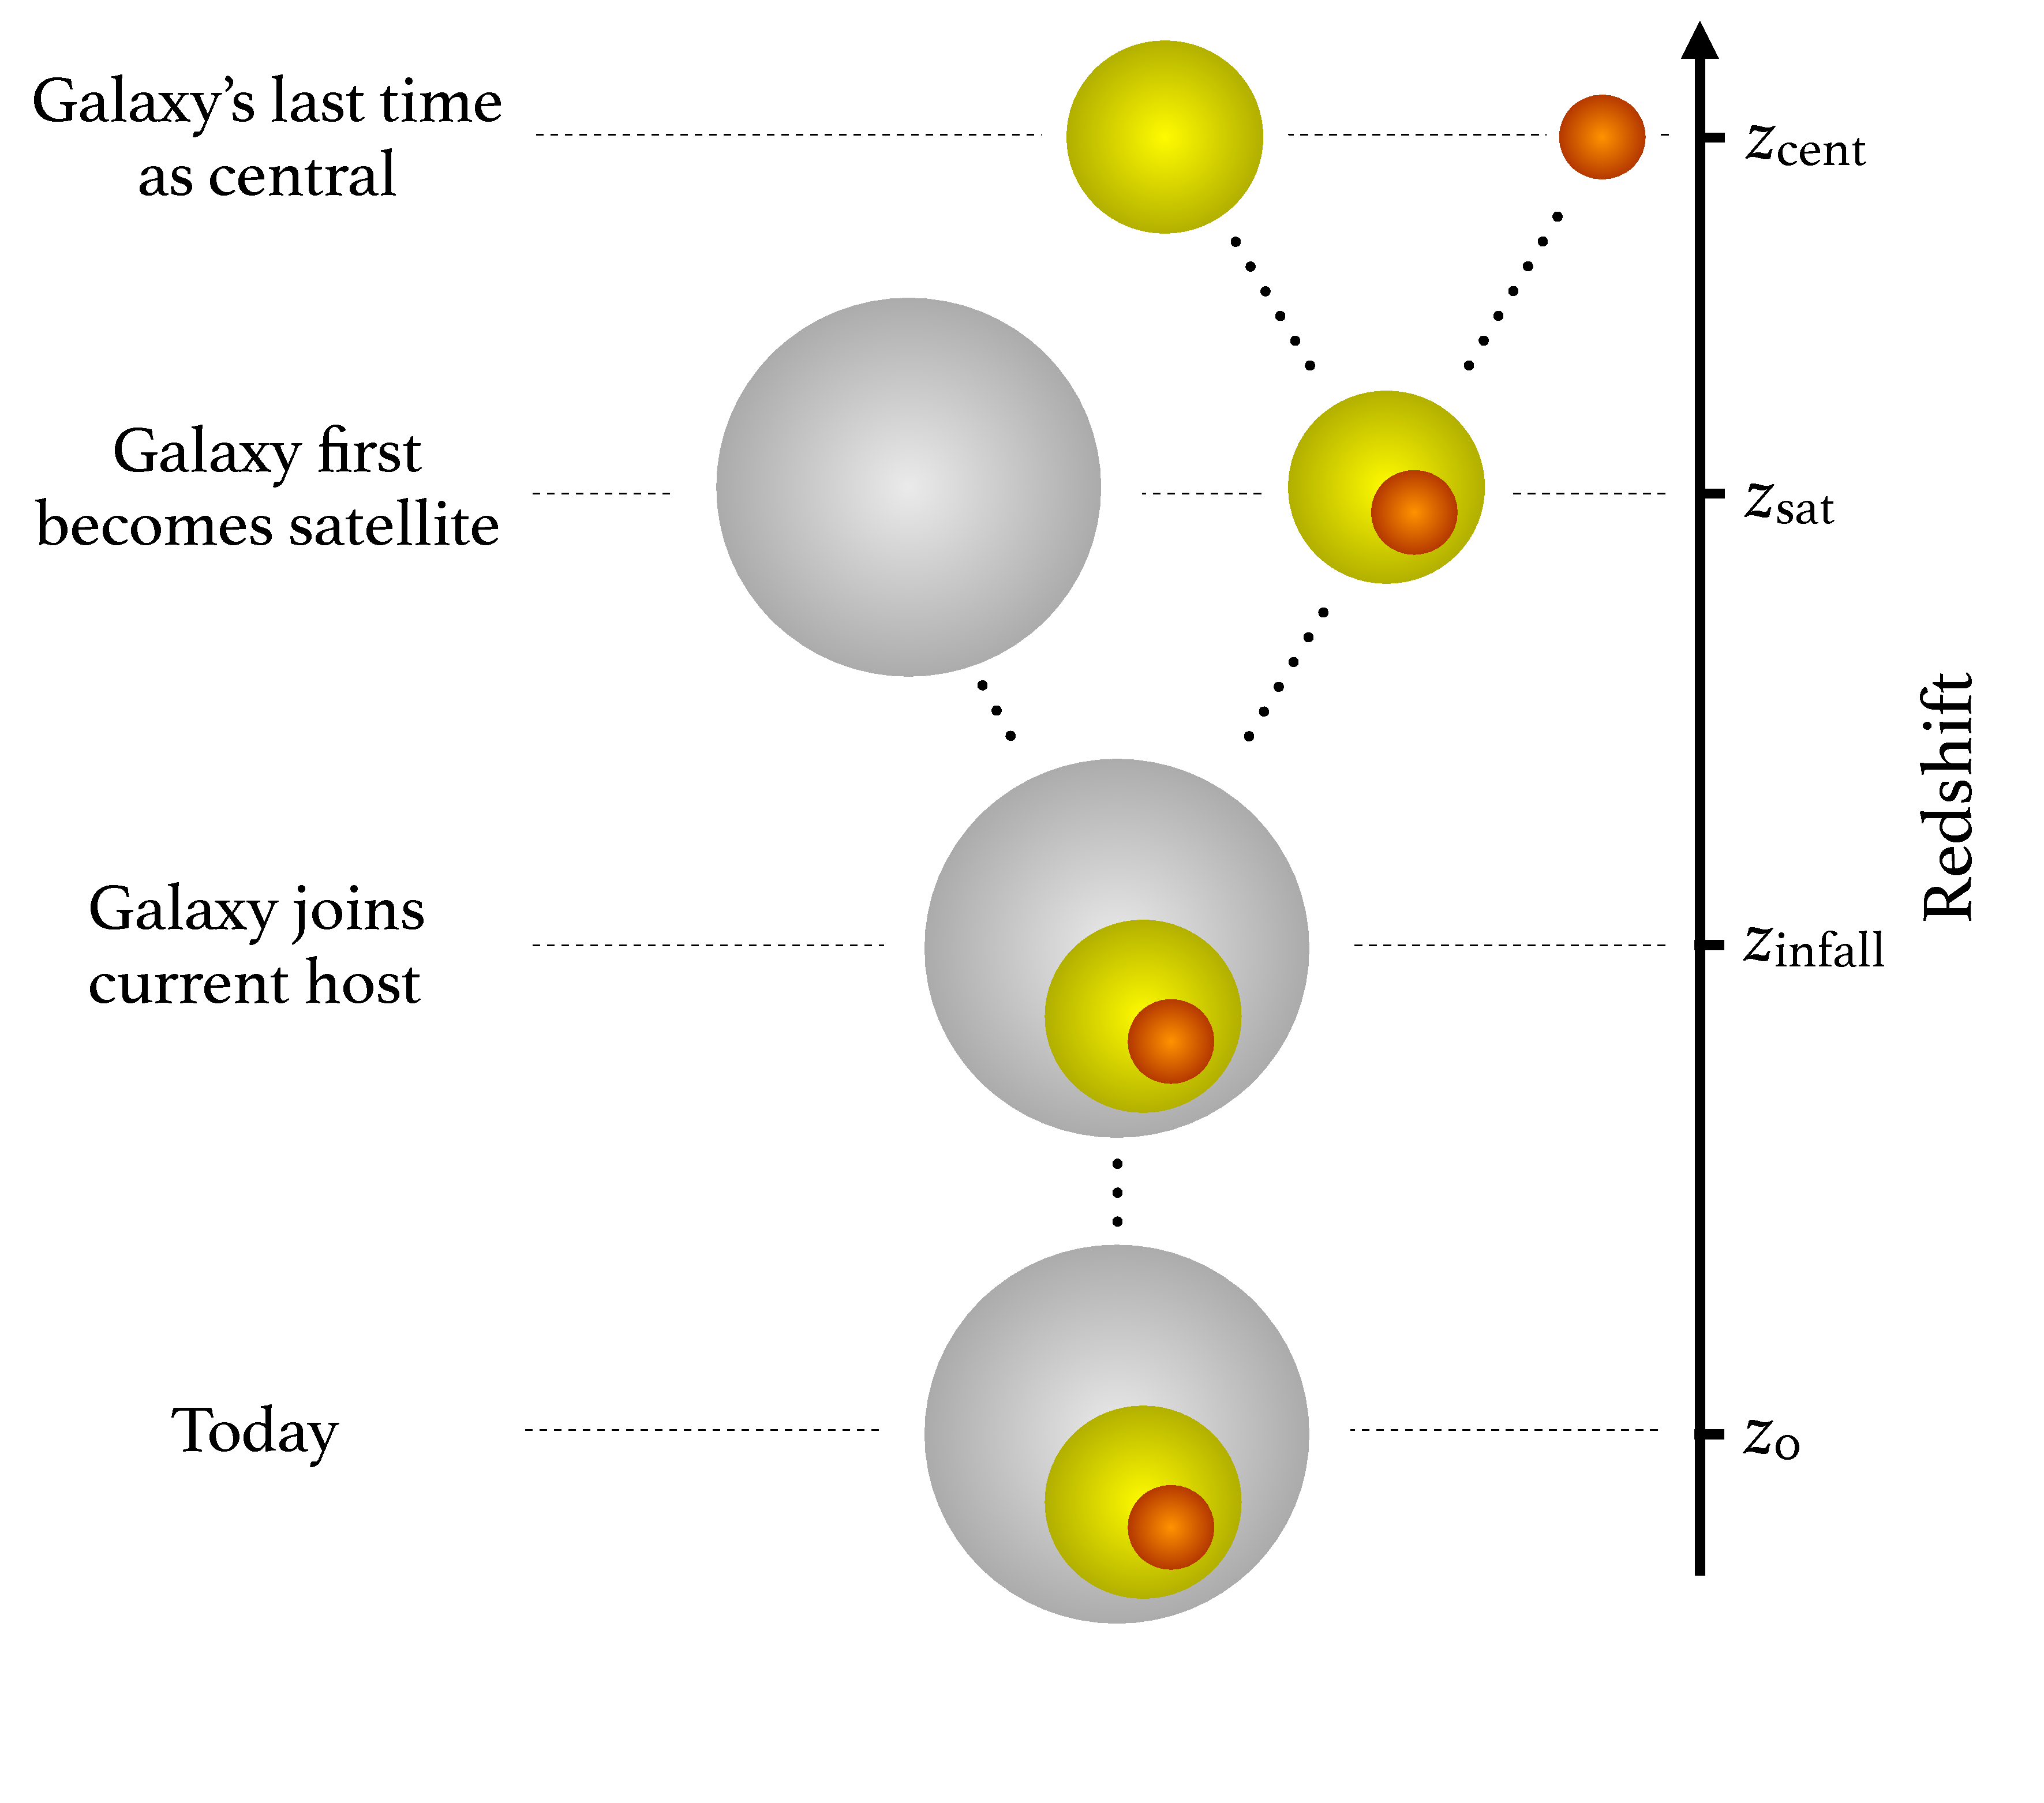
\includegraphics[width=\linewidth]{history_chart.pdf}}
%\caption{Schematic figure showing the relevant times we consider in this work. The brown circle represents a galaxy of interest, which is a satellite at redshift $z_0$, part of a host group shown in grey. We identify the last redshift at which the brown satellite was hosted by the grey host as $\zinfall$. The last time at which the brown satellite was a central galaxy is labelled $\zcent$. When the brown satellite fell into the grey host (identified at present with \texttt{GroupID}), it may in fact have already been part of another group, shown in green. If this is the case, then $\zcent \neq \zinfall$.}
%\label{f:history_chart}
%\end{figure}


\section{Present-day cluster galaxies in \eagle}

\begin{itemize}
  \item make a plot similar to \Cref{f:shmr_now} but showing how this depends on the subhalo-to-host mass ratio (e.g., with different lines, or normalizing an axis or both axes)
  \item also make a plot with total-to-stellar mass ratio as a function of cluster-centric distance (also showing the effect of host halo mass)
  \item also have a look at scatter in mtot vs.\ mstar
\end{itemize}


\subsection{The relations between total and stellar mass}

\Cref{f:shmr_now} shows the stellar-to-halo mass relation (SHMR) and the halo-to-stellar mass relation (HSMR)\footnote{Note that due to intrinsic scatter, one cannot be obtained by simply inverting the other.} Central and satellite galaxies clearly follow different relations. This result has been seen for a long time in simulations and originates in the severe tidal stripping suffered by satellite galaxies (moreover, with time, some of the stripped mass will be accreted by the central subhalo). The ratio between the relations for centrals and satellites is approximately constant in both stellar mass (for the HSMR) and subhalo mass (for the SHMR),
\begin{align}\label{eq:relation_ratios}
  \Mtotal^\mathrm{sub}(\mstar) 
      &= \upsilon_\mathrm{HSMR}(\mstar) \Mtotal^\mathrm{cen}(\mstar) \\
  \log \upsilon(\mstar) &= XXX + YYY \log \mstar
\end{align}
and


We also show two observational results for comparison: the central HSMR by \cite{vanuitert16}, and the satellite HSMR by \cite{sifon18_meneacs}. There is general agreement between the observational results and \eagle, with perhaps some evidence for larger total satellite masses at large stellar masses in EAGLE compared to observations, which \cite{sifon18_meneacs} showed is also seen in the \subfind\ subhalo catalogue of EAGLE \citep{}.

\Cref{f:shmr_mu} shows the dependence of the HSMR on host halo mass. As seen in the right panel, there is a slight dependence of the HSMR with host halo mass, with more massive haloes hosting satellites with a lower total-to-stellar mass ratio (i.e., a lower dark matter fraction). This can easily be understood by the effect of tidal stripping from the host halo, which is more severe in more massive hosts and affects dark matter more strongly than stellar mass \citep[e.g.,][]{}. 

In order for the EAGLE SHMR to be useful for halo model interpretations of lensing or clustering measurements, we fit the HSMR with a double power-law in total mass, modulated by host halo mass:
\begin{equation}\label{eq:shmr_Mh}
%  \msub(\mstar,\Mhost) 
%    = m_0(\Mhost)
%      \frac{\left(\mstar/m_1\right)^{\beta_\mathrm{s}^\star}}
%           {\left[1+\left((\mstar/m_1\right)
%                 {\beta_\mathrm{s}^\star-\gamma_\mathrm{s}^\star}\right]}
  \mstar(\msub,\Mhost)
    = m_{\star,0}^\mathrm{sub}(\Mhost)
      \frac{\left(\msub/m_1^\mathrm{sub}\right)^{\beta_1^\mathrm{sub}}}
           {\left[1+\left(\msub/m_1^\mathrm{sub}\right)\right]
                 ^{\beta_1^\mathrm{sub}-\beta_2^\mathrm{sub}}
           }
\end{equation}
where for simplicity we model $m_{\star,0}$ as a power law:
%\begin{equation}\label{eq:m_0}
% \log m_0(\Mhost) = a_\mathrm{h} + b_\mathrm{h}\log \Mhost \,.
%\end{equation}
\begin{equation}\label{eq:mstar_0}
 \log m_{\star,0}^\mathrm{sub}(\Mhost) = a_\mathrm{0} + b_\mathrm{0}\log \Mhost \,.
\end{equation}
\comment{we would have to decouple this from the mass function in order to be consistent with the halo model. Can do this by fitting individual $\msub$s with this equation, though maybe too much?}
\comment{We find that the following parameters represent the data well:}


The left panel of \Cref{f:shmr_mu} shows the same relations but separated by the ratio of satellite-to-host mass,
\begin{equation}\label{eq:mu}
  \mu \equiv \frac{\msub}{\Mhost} \,.
\end{equation}
The HSMR depends more strongly with $\mu$ than $\Mhost$ alone. Furthermore, we find that the HSMR flattens at smaller $\mu$. This

\comment{To highlight this, we show the HSMR as a function of the distance from the subhaloes to the host halo centre of mass in \Cref{fig:hsmr_R}.}


\begin{figure*}
  \centerline{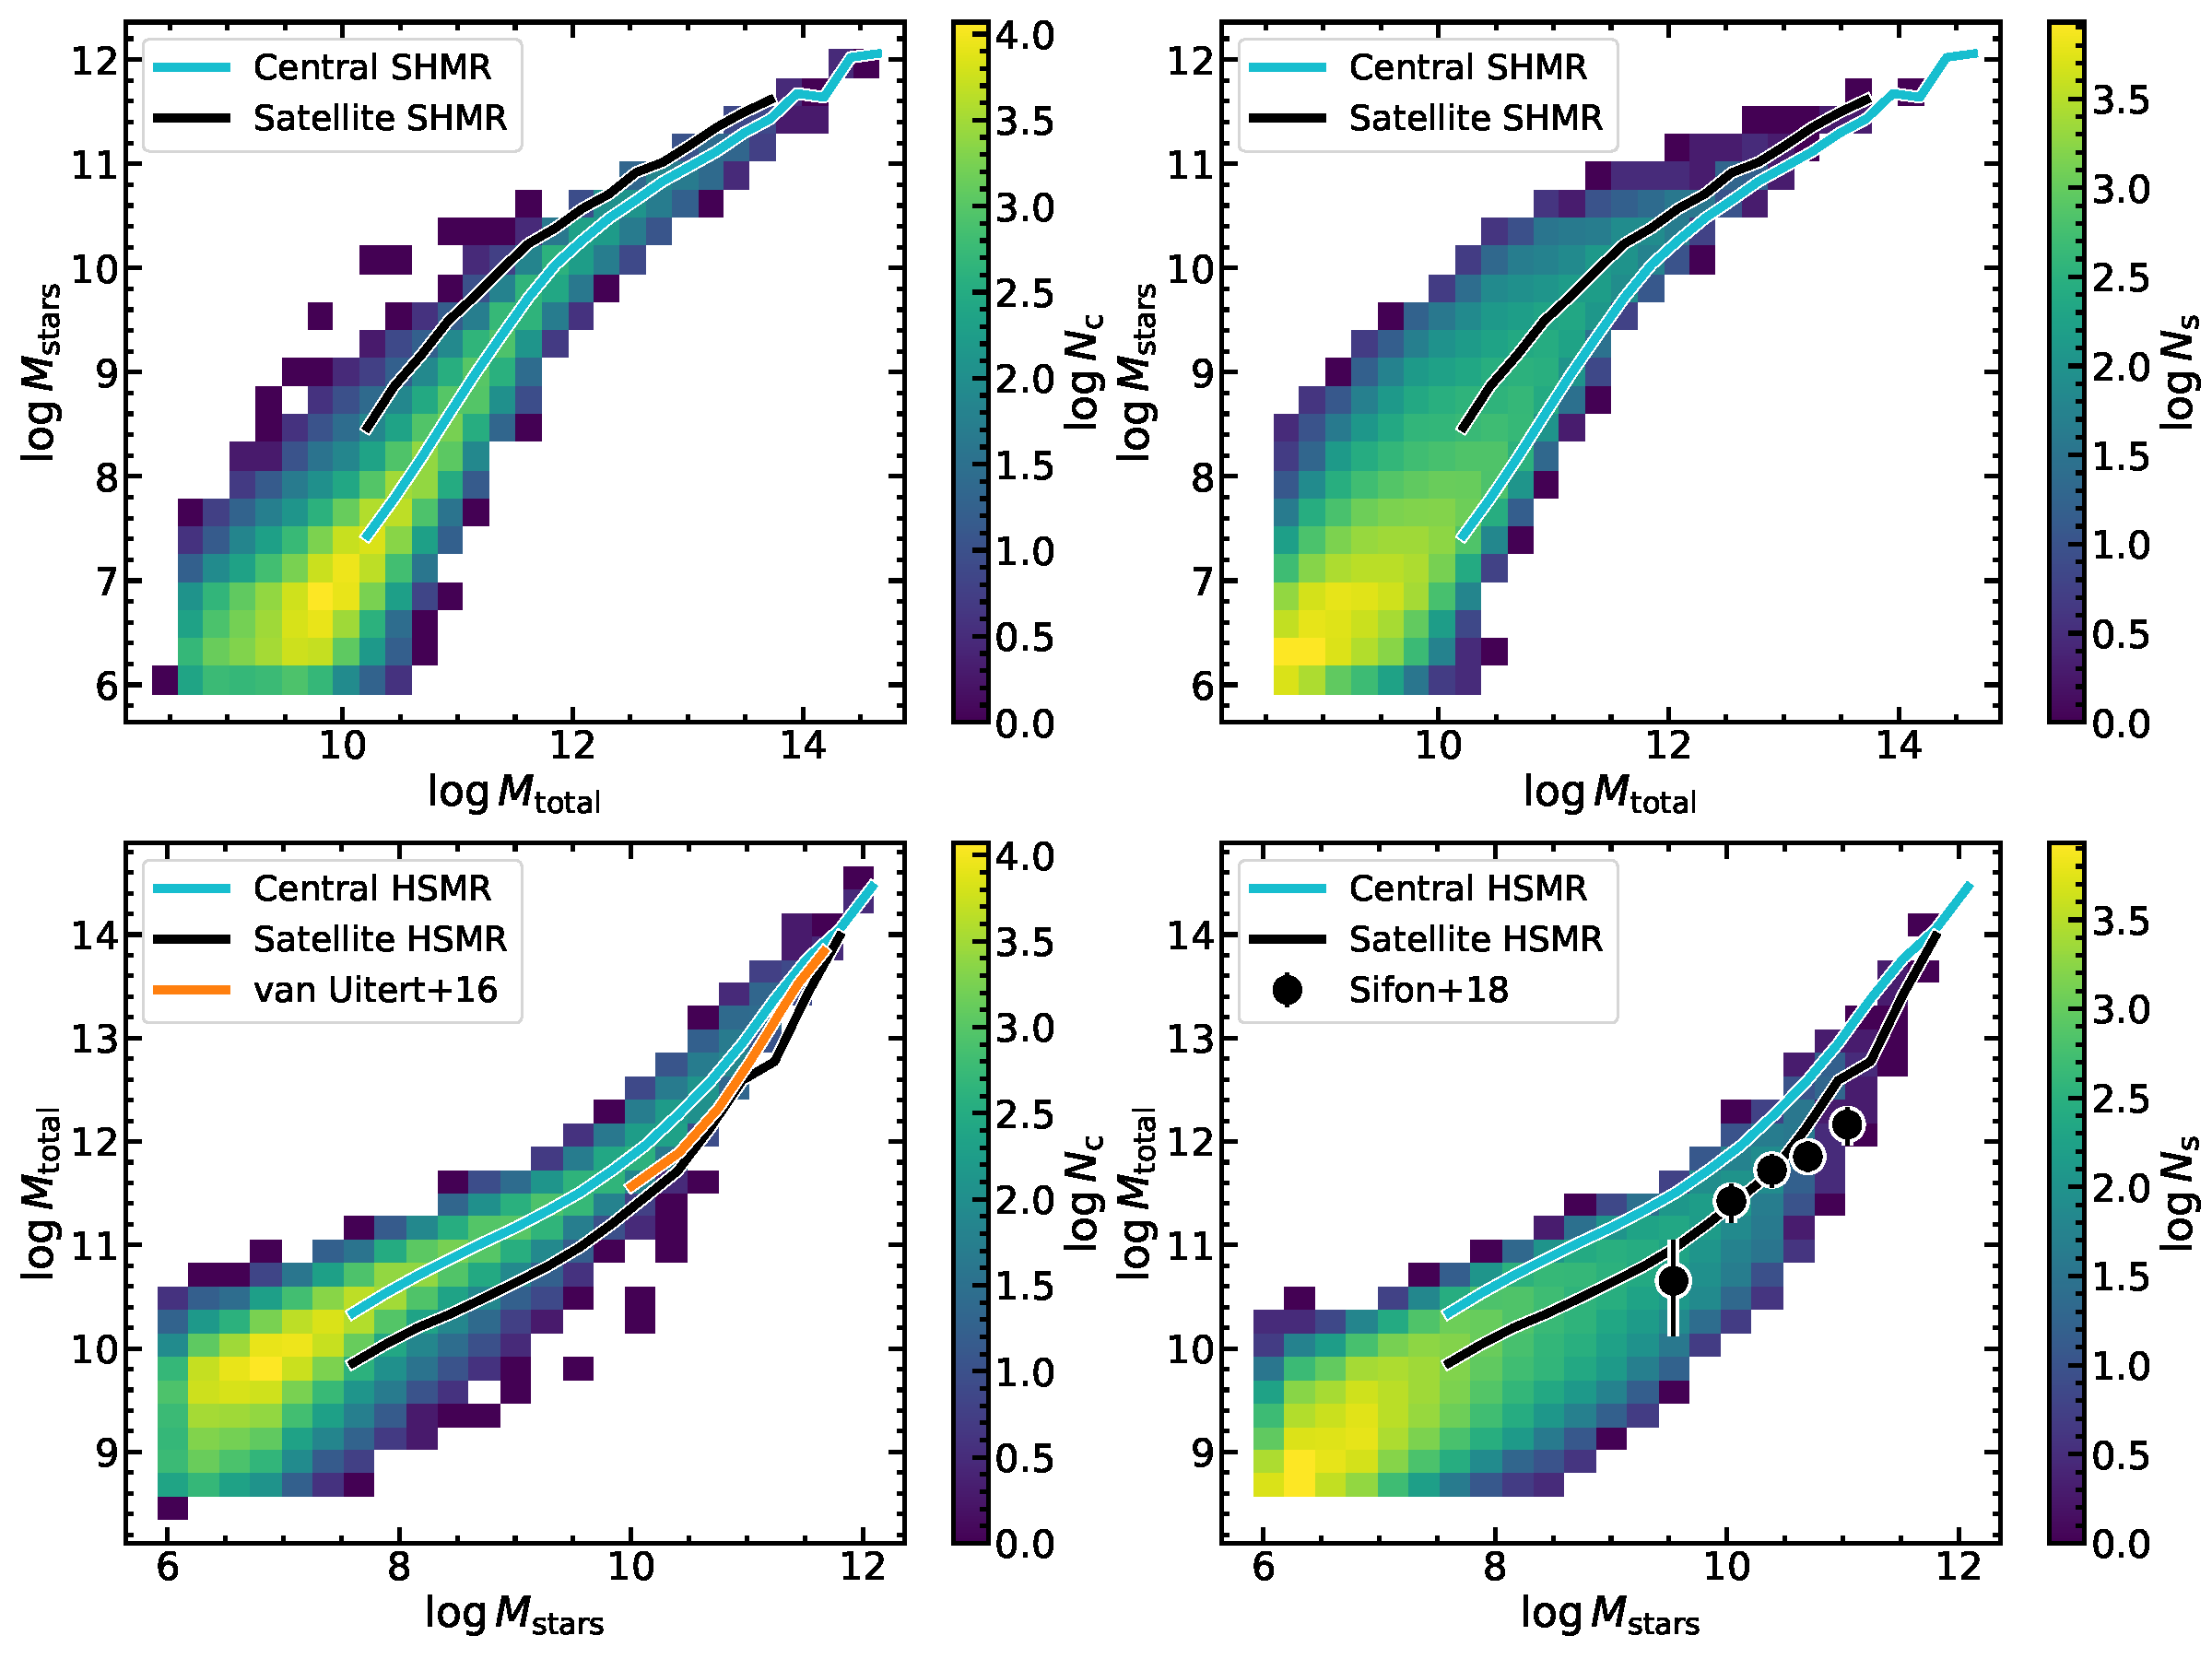
\includegraphics[width=\linewidth]{shmr_censat.pdf}}
  \caption{The stellar-to-halo mass relations (SHMR, top panels) and halo-to-stellar mass relations (HSMR, bottom panels) for central (left panels) and satellite (right panels) cluster galaxies in \eagle. Color scales represent the log of the number of central and satellite galaxies, respectively, and lines are the means in each panel, as labelled, and are only shown where the samples are complete in the independent (i.e., x-axis) variable. Central total masses refer to $M_\mathrm{200m}$, while subhalo masses are total \hbt\ masses. The central HSMR is compared to that derived from KiDS data by \citet{vanuitert16}, while the satellite HSMR to that measured in MENeaCS clusters by \citet{sifon18_meneacs}.}
  \label{f:shmr_now}
\end{figure*}

\begin{figure*}
  \centerline{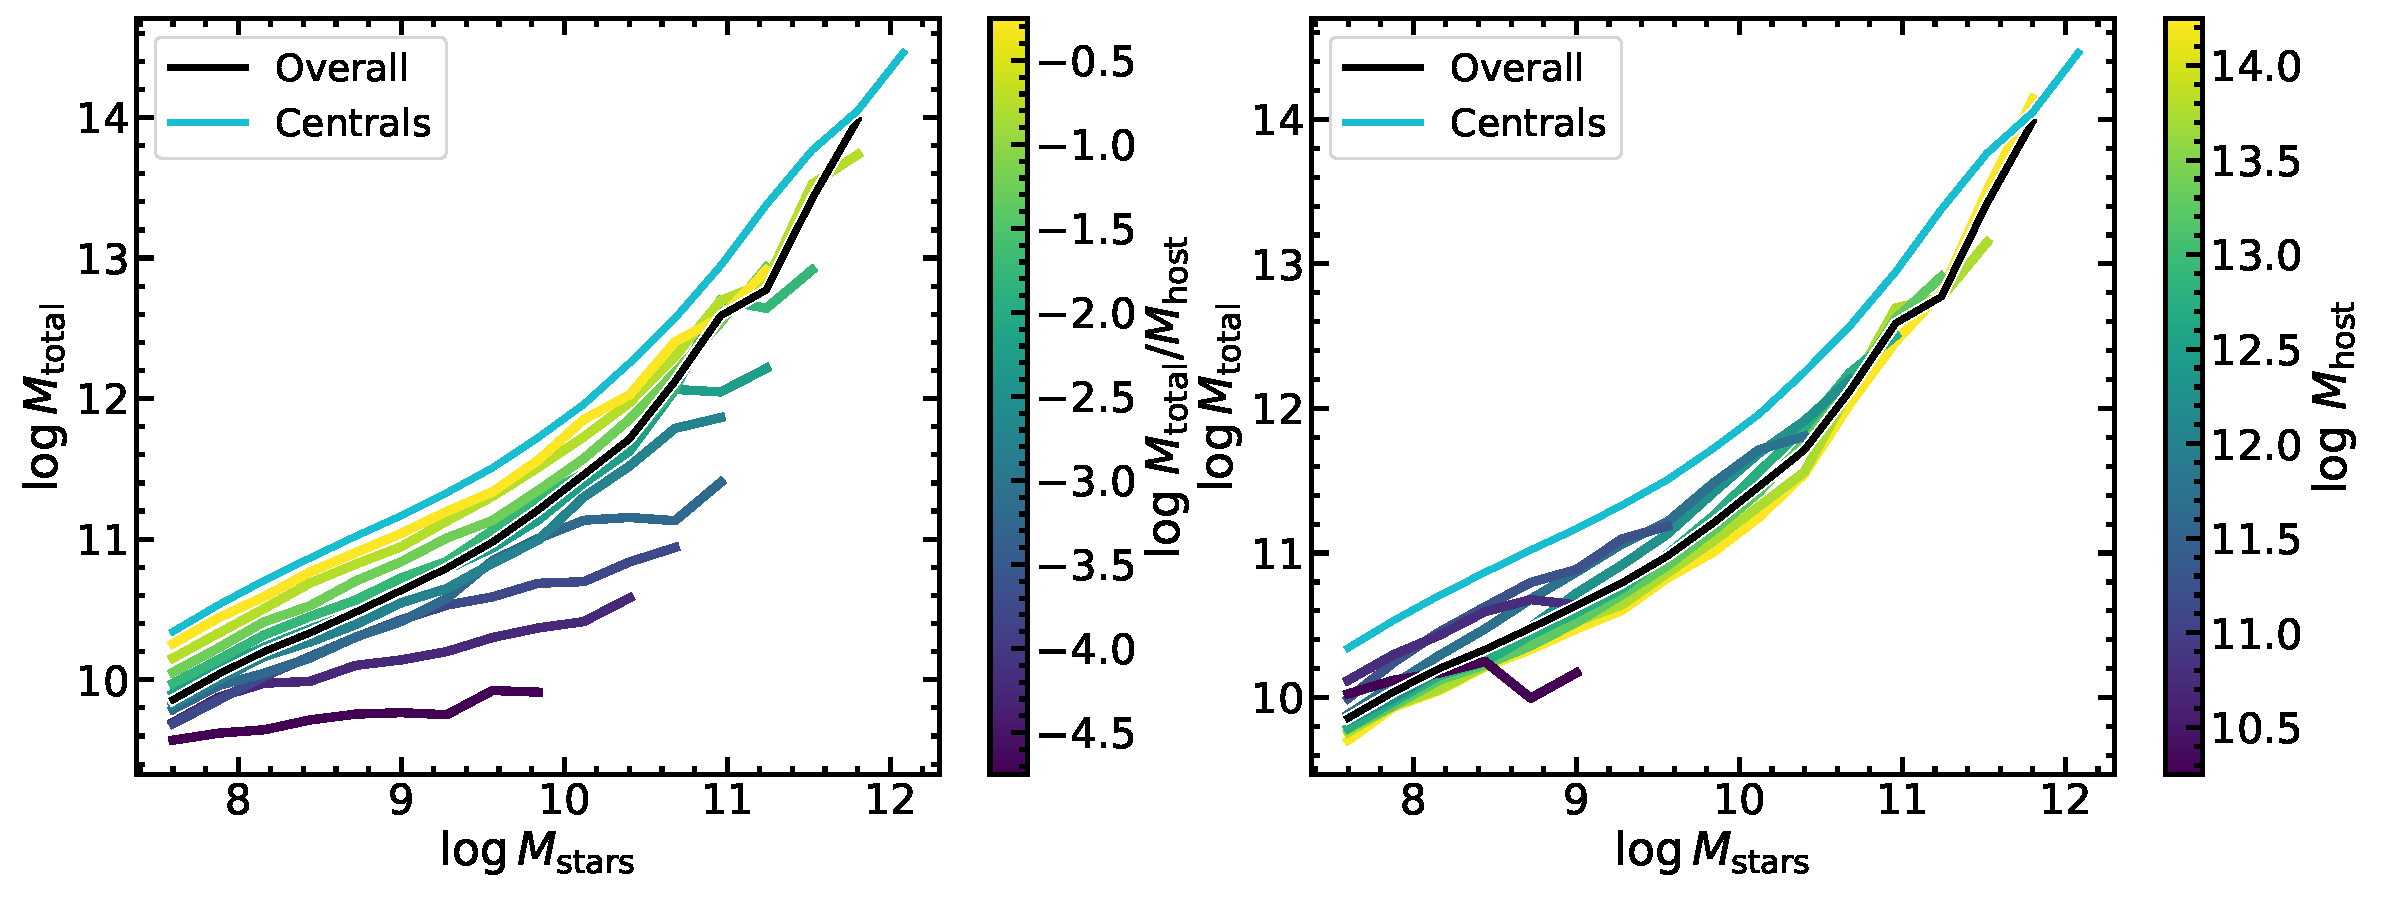
\includegraphics[width=\linewidth]{shmr_mu.pdf}}
  \caption{The dependence of the halo-to-stellar mass relation on subhalo-to-host mass ratio (left) and on host halo mass (right). The black line shows the HSMR averaged over all subhaloes, while the cyan line shows the HSMR of centrals for reference. Mass definitions are as in \Cref{f:shmr_now}. \comment{check number of particles/destruction rate vs.\ mu}}
  \label{f:shmr_mu}
\end{figure*}


\subsection{Subhalo disruption}

Recently, it has become apparent that most, if not all, disruption of subhaloes in N-body  simulations is a result of numerical noise or other artefacts of the simulation, rather than it being the consequence of physical effects \citep{vdbosch18_analytic,vdbosch18_nbody}. In this section, we present demographics of disrupted subhaloes in \eagle; in \Cref{s:lensing} we discuss the implications of their demographics for comparisons with observational measurements.

\comment{\Cref{fig:} shows the fraction of disrupted subhaloes as a function of host mass. Use Frank's papers as reference - are things consistent? do we learn anything?}


\section{The evolution of cluster galaxies}

\begin{itemize}
  \item reproduce the 2d histograms in \Cref{f:shmr_now} but now show tracks for a few subhaloes, i.e., how do they move along this plane as they are accreted and orbit the cluster?
  \item show something like the fraction of subhaloes that were centrals at infall (i.e., $\tcent = \tinfall$) as a function of halo mass, subhalo mass, and infall time.
  \item follow up the 4-panel shmr figure with relations with time. Perhaps we can find a time when central and satellite galaxies had the same HSMR? What are the roles of stripping and star formation in this evolution?
\end{itemize}

\begin{figure*}
  \centerline{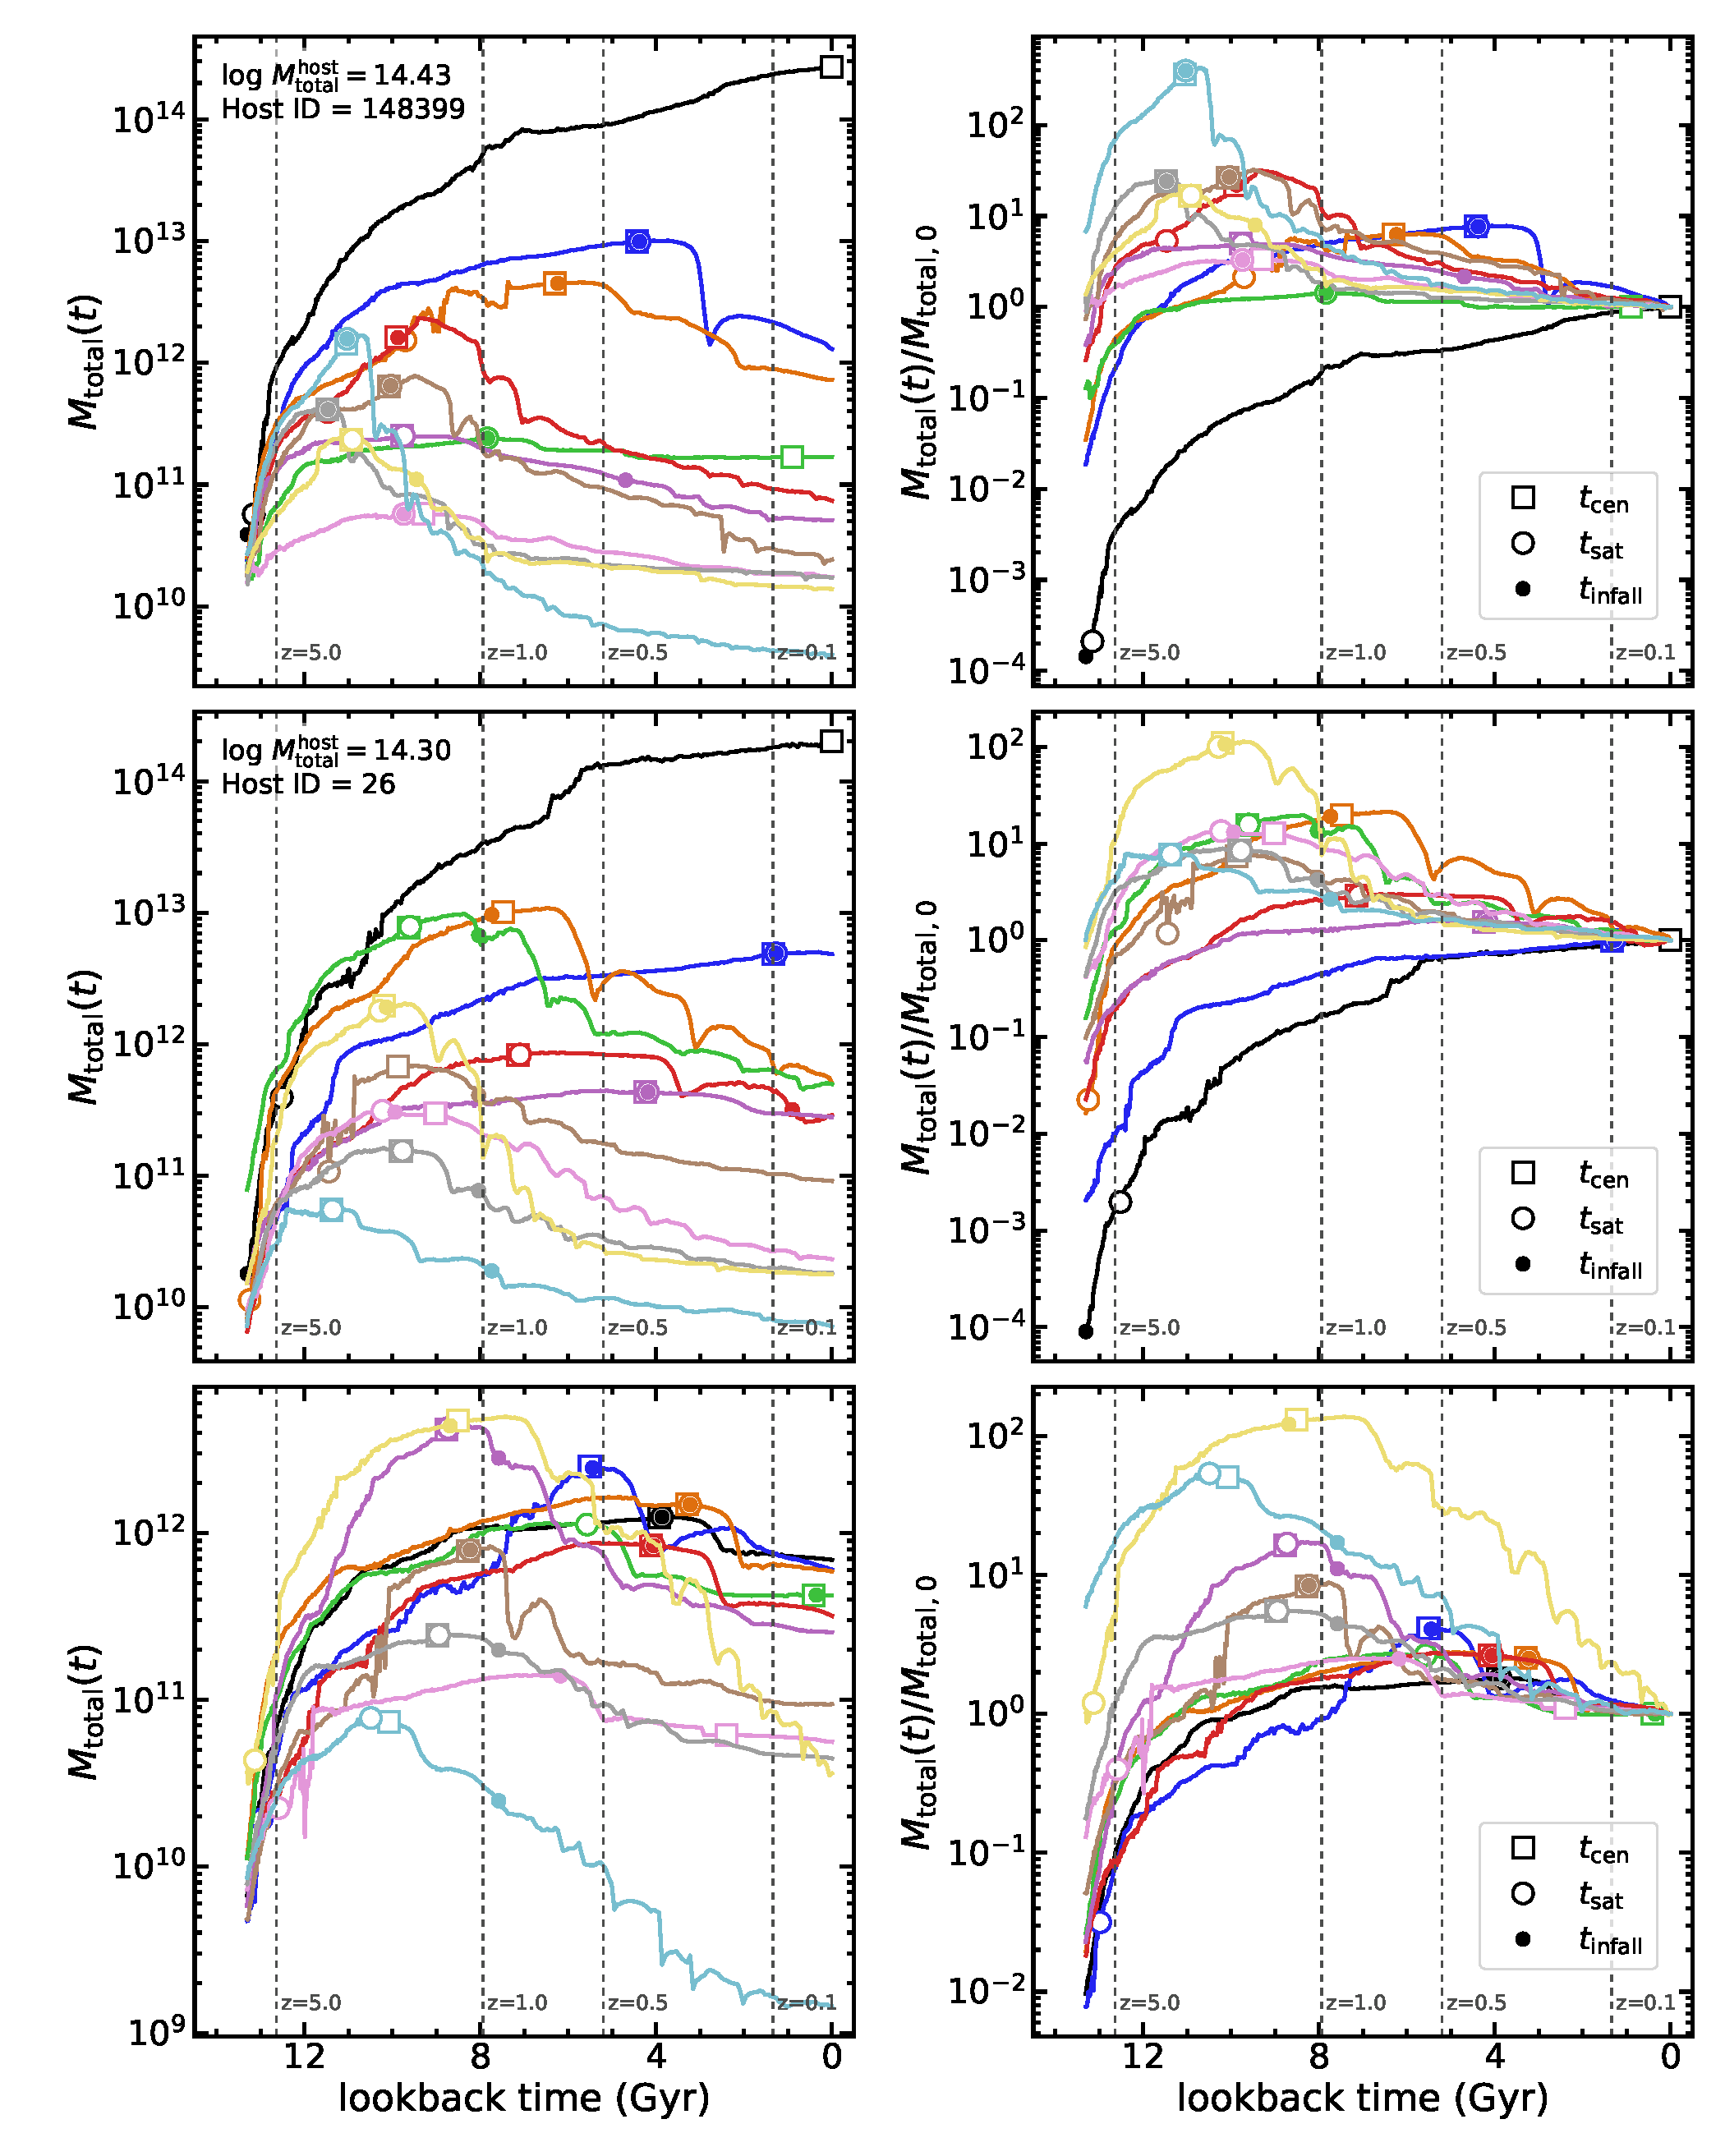
\includegraphics[width=\linewidth]{track_Mtotal.pdf}}
  \caption{The evolution of the total mass of the 11 most massive subhaloes (i.e., the central plus the ten most massive satellite subhaloes) in the three most massive haloes in \eagle. Empty squares, empty circles, and filled circles correspond to the first time a subhalo became a satellite ($t_\mathrm{sat}$), the last time it became a central ($t_\mathrm{cen}$), and the time of infall to its current host ($t_\mathrm{infall}$), respectively. The left panel shows mass as a function of lookback time, while the right panel is normalized by present-day mass. Each subhalo has the same color in the left and right panels.}
  \label{fig:track_Mtotal}
\end{figure*}

\noindent
Notes on \Cref{fig:track_Mtotal}.
\begin{itemize}
  \item In general, we'd expect $i_\mathrm{cen} = i_\mathrm{sat} - 1$, i.e., a subhalo is a central right until it becomes a satellite, after which it is never central again. That's in general not quite what we see.
  \item The steeper growth of the central subhaloes is not reflected in a comparable decrease in the mass of the most massive subhslaos. Where is all this mass in the last $\sim$8 Gyr coming from?
  \item Note that all subhaloes which lose mass abruptly (e.g., yellow, cyan in top row) then regain some mass. This is expected as the subhalo `re-virializes'
  \item Funny that all centrals \emph{were} satellites at some point (probably only one snapshot?)
  \item The earliest accreted subhaloes -- cyan in row 2 and grey in row 3 -- have had multiple severe mass loss episodes, as expected.
  \item some (potentially) interesting summary plots:
%  \begin{itemize}
%    
%  \end{itemize}
\end{itemize}

\subsection{The impact of tidal stripping on the relation between total and stellar mass}

Possible plots:
\begin{itemize}
  \item HSMR for different redshifts
  \item HSMR for different times-since-accretion
\end{itemize}

%\begin{figure*}
%  \centerline{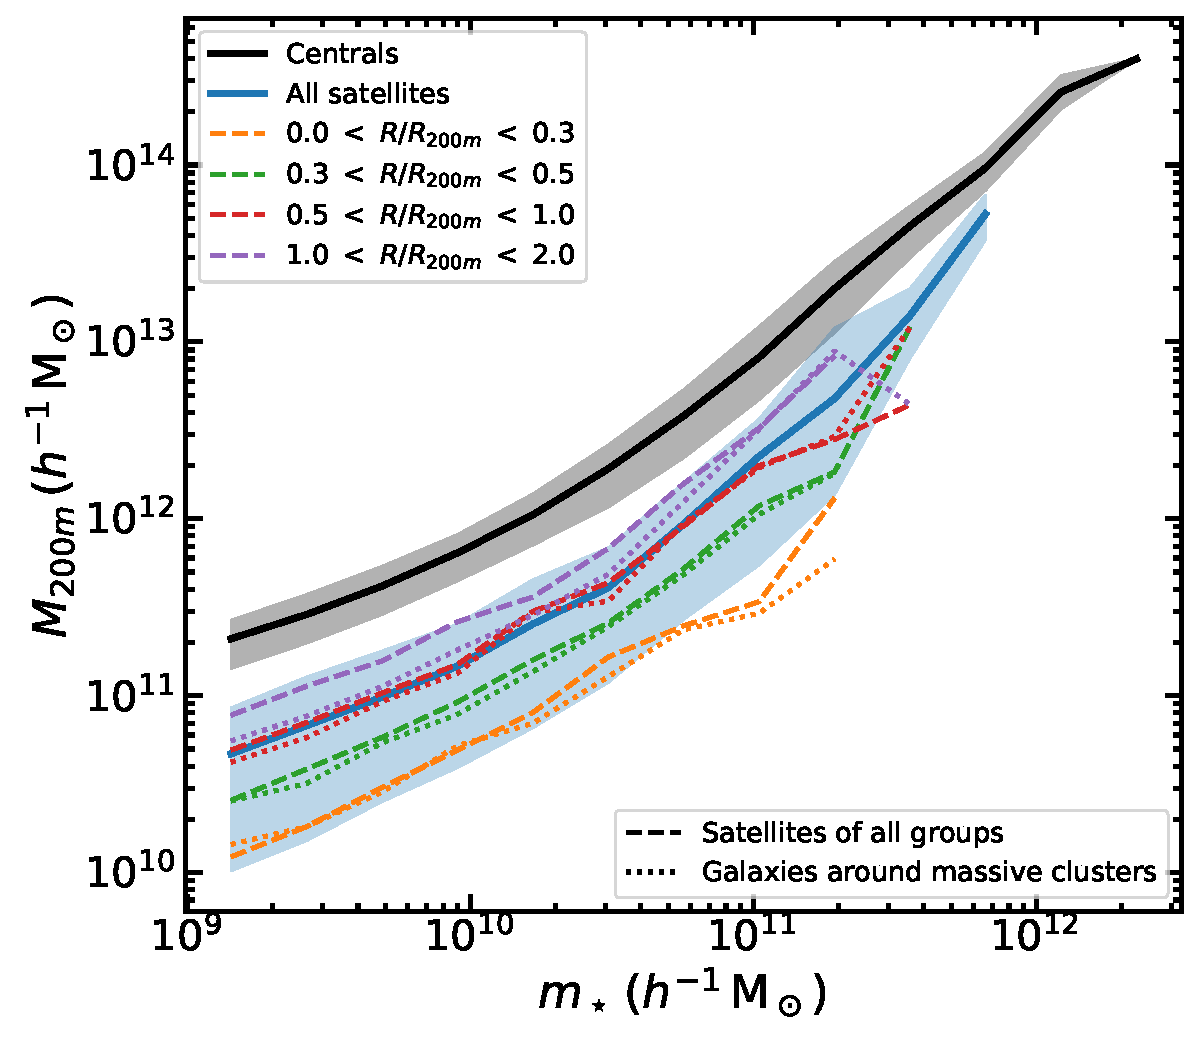
\includegraphics[width=\linewidth]{total_to_stellar_groups_and_clusters.pdf}}
%\caption{The total-to-stellar mass relation of galaxies as a function of distance to their \emph{host} group (dashed lines), and as a function of their distance to the \emph{nearest} massive ($M_{200m}>10^{13}\,h^{-1}\,\Msun$) cluster (dotted lines), each normalized by the size of the group/cluster. The blue line shows the average total-to-stellar mass relation of all satellites belonging to all groups, and the black line shows the total-to-stellar mass relation of central galaxies. In the latter two, the respective shaded regions show the scatter in each.}
%\label{f:relation}
%\end{figure*}

%\Cref{f:relation} shows that:
%\begin{enumerate}
%  \item the TSMR of subhaloes is approximately a factor 4 lower than that of centrals.
%  \item the TSMR decreases in amplitude as we get closer to the cluster centre, but its shape does not change.
%  \item If cluster size is accounted for, the TSMR of subhaloes does not depend on cluster mass (i.e., dashed and dotted lines of the same color overlap), except perhaps for low-mass galaxies outside $R_{200m}$. \emph{This suggests that massive clusters exert their influence out to larger radius compared to low-mass clusters}, especially for low-mass galaxies ($m_\mathrm{gal}\lesssim10^{-2}M_\mathrm{cl}$).
%\end{enumerate}

%Caveats:
%\begin{enumerate}
% \item Need to check how much of point (ii) may be caused by biases in subfind (compare to the curve of recovered versus true mass as a function of radius from Knebe+11).
% \item Remove centrals of massive groups from the coloured curves.
% \item Remember that Marco showed that the satellite fraction is really off in \eagle\ (compared to GAMA), so should not mix centrals and satellites, nor take the satellite fraction seriously (?).
% \item It seems like the subfind bias is pretty large and may be driving most if not all the changes we see as a function of $R$. Perhaps I could gauge this bias by comparing an \eagle\ DM only sim with a DM only Rockstar catalog? Even then, baryonic effects on density profiles could conceivably change the comparison.
%\end{enumerate}


%\section{Application to satellite lensing measurements}\label{s:lensing}
%
%This may be worth another paper where we look at more observational stuff: phase-space, ESD, etc




\bibliographystyle{mnras}
\bibliography{bibliography}






\end{document}


